\subsubsection{Sort}
The Sort controller lets user perform the Quicksort and Mergesort algorithms on arrays.
\begin{figure}[h]
    \centering
    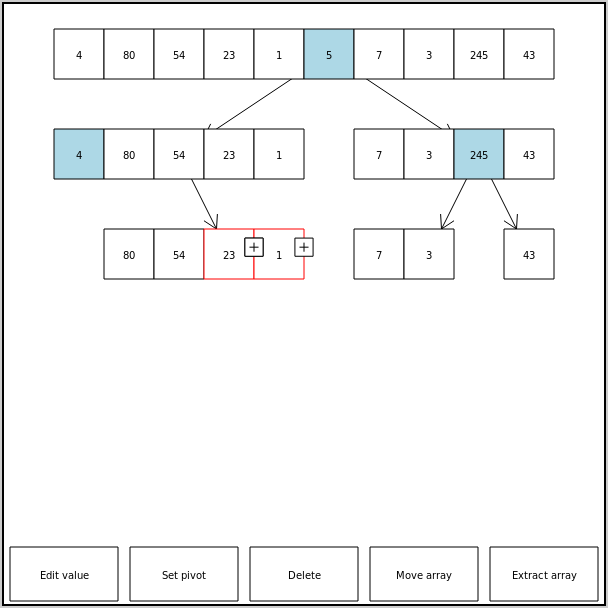
\includegraphics[width=0.75\linewidth]{/graphdrawer/sortui}
    \caption{Sort - user interface}
    \label{fig:graphdrawerSortUserInterface}
\end{figure}
\\[11pt]
The following properties can be determined by the optional configuration object:
\begin{enumerate}
    \item \code{sortType}, determines which algoritm to use. Can either be \code{"Mergesort"} or \code{"Quicksort"}. The default value is \code{"Quicksort"}.
    \item \code{bsf}, button-size-factor, determines how large the "+" buttons between nodes are. The default value is 3.
    \item \code{pivotColor}, determines which fill color nodes which are marked as pivot will have.
    \item \code{selectedColor}, determines which stroke color nodes which are selected will have.
    \item \code{extractType}, determines node position relative to other nodes when extracting nodes from an array. Possible values are \code{"vSorter"} which means the nodes are positioned based on their value, from low to high, and \code{"xSorter"} which poisitions them based on their x-position in the world.
    \item \code{joinType}, determines node position relative to other nodes when joining the nodes from different arrays to a new array. Possible values are \code{"vSorter"} and \code{"xSorter"}.
    \item \code{steps}, which contains information about the starting array which the student needs to sort. It can also contain information about all of the actions one of the algorithms perform to sort the array.
\end{enumerate}
The \code{mouseDownHandler} function has four parts. It will first check if the world is empty. If it is, the first click will create the first node and array. If it is not empty, then it will check if any of the buttons were clicked. The buttons can only be clicked if they are visible, and they are made visible when the user selects one or more nodes. Only one node can be selected, but several can be in the selection list. When the user selects a node, the "Edit value", "Set pivot" and "Delete" buttons are shown. If the selection list contains node from only one array, the "Move array" and "Extract array" buttons are also shown. If the \code{sortType} is \code{"Mergesort"} and the selection list contains nodes from at least one array, then the "Join" button is also shown. If no button is clicked, and the user is trying to move an array, the array will be moved to the position of the interaction event. Finally, if nothing else happened, the selected node and the selection list is updated based on which nodes the user interacts with. When the user clicks and holds down their mouse button, the controller will start tracking which nodes are under the cursor. When the button is released, any node which was under the cursor will be in the selection list, and the last node from the list will be the selected node.
\\[11pt]
Arrays doesn't exist in the GraphDrawer world. They are therefore only a part of the Sort controller. The controller has a reference to an array of array objects. The array objects contain a reference to every node in the array, the position of the array, and an list of other arrays which the array has a connection to. When an array is created, its position is set to the position of the first node. This is done so that the array won't move when more nodes are added to it. When a node is added to the array, all of the other nodes in the array will have an invalid position. To fix this, the node is first placed at the correct index, and then every node in the array is positioned according to their index in the reference array. When a node is removed, the same steps are performed. Because arrays doesn't exists in the GraphDrawer, edges between them also doesn't exist. Any link between two arrays, is really an edge between the nodes closest to the center of the arrays. 